\chapter{Methods and Implementation}
This chapter focuses on the experimental design and implementation of the artefact,
covering the self-imposed project management methodology, original concept design 
and the overall development process.

\section{Methodology}
When developing software, there are a wide variety of available options to manage the development 
process, which help to structure how time should be allocated as development progresses. 

\subsection{Waterfall} 
\para The first methodology considered was the Waterfall methodology, which is a very common 
approach to software development being sometimes referred to as the Software Development Life Cycle, or SDLC \autocite{adobePopularProjectManagement2023}.
Waterfall is a highly structured and strict methodology which enforces that one stage of development must be completed before the next can begin,
which creates a cascading set of steps, hence its namesake.

\begin{figure}[H]
    \centering
    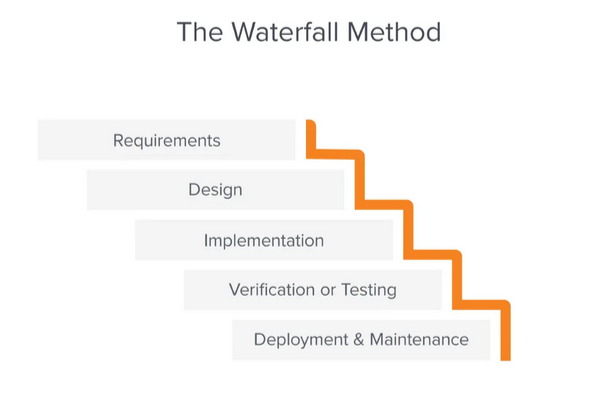
\includegraphics[width=0.8\textwidth]{Implementation/Methodology/Waterfall.png}
    \caption{An overview of a Waterfall workflow \autocite{adobeWaterfallMethodologyProject}. \label{fig:Waterfall}}
\end{figure}

\noindent Waterfall begins by ascertaining all project requirements for all stages of the project, which 
would include costs, risks, associated dependencies and overall timelines for completions of each stage.
Following this is the design stage, where a general high-level design is created to demonstrate the 
project, and this design is then acted upon and implemented in the implementation stage. Then, the 
implementation is rigorously tested before its eventual deployment.

\para It is a methodology with a strong reputation due to its clear structure, with all necessary facts and figures 
being calculated in the requirements stage before any designs or development occur. The clear structure allows 
progress to be easily measured against each predefined milestone.

\para Though, despite these advantages, Waterfall brings with it some clear disadvantages - the first of which 
being that with all requirements being defined at the very beginning of the project's development,
it introduces significant difficulty should there be any further requirements specified during development. This would also 
bring in the second disadvantage known as 'deadline creep' \autocite{adobeWaterfallMethodologyProject}; 
if one stage is delayed, such as by request for additional features, this would then impact all subsequent stages. 

\subsection{Agile}
The second methodology considered was another highly reputed software development methodology known as Agile.
Unlike Waterfall which defines all stages and requirements at the beginning, Agile is a highly iterative methodology with steps
known as 'sprints' which are frequently repeated, providing a more incremental approach to development. Each of these sprints
would represent a small part of the program, eventually building up to the full version.

\para As depicted in Figure \ref{fig:ExampleAgileSprint}, 
Agile sprints begin by planning the overall aims of that particular sprint. Similarly to Waterfall, a high-level
design is then created and developed, before being rigorously tested. This is also one of Agile's key benefits; the 
constant testing of the small parts developed in each sprint helps ensure that all bugs can be rectified, unlike 
Waterfall where the whole product is tested and some smaller elements with bugs could potentially be overlooked.
After testing, the product of that sprint is deployed and reviewed. Then, the cycle begins anew with another 
sprint.

\begin{figure}[H]
    \centering
    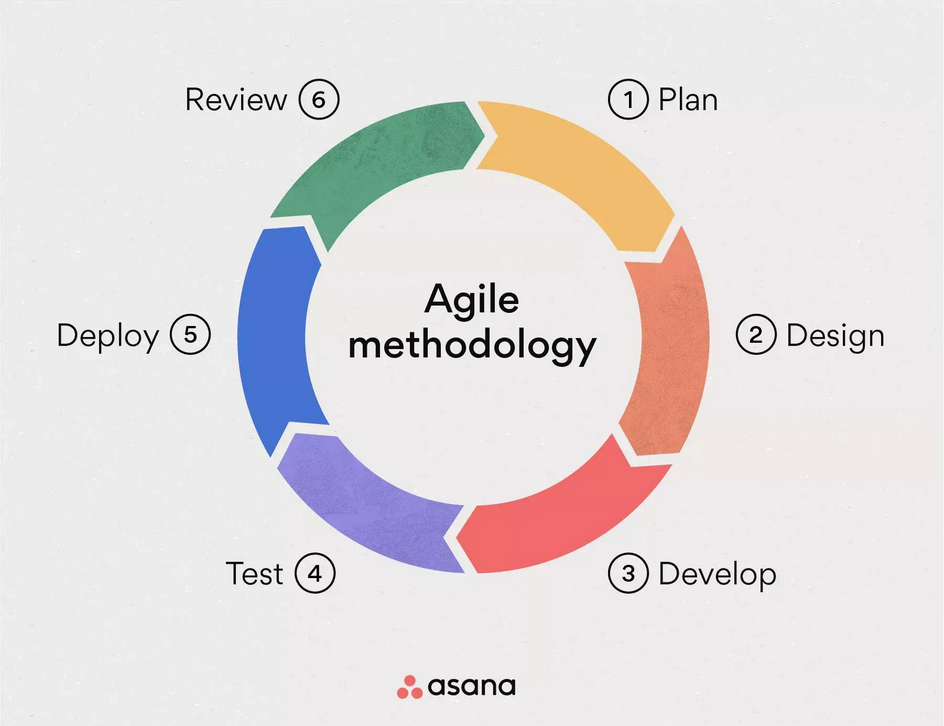
\includegraphics[width=0.65\textwidth]{Implementation/Methodology/Agile.png}
    \caption{An overview of an Agile sprint \autocite{asanaWhatAgileMethodology}\label{fig:ExampleAgileSprint}}
\end{figure}


\noindent The most prominent key benefit of Agile is its sprint-based iterative nature that allows for requirements to shift 
throughout development without major disruption. Furthermore, this incremental process minimises the risk of total project 
failure as usable components are constantly produced. In business environments, Agile also allows for enhanced teamwork, though 
this will not be present in this particular project.

\para As with Waterfall, Agile is not without drawbacks. Agile's most notable drawback is known as 'scope creep' \autocite{malsamWhatScopeCreep2024},
which occurs when requirements are continually added to a point where development can never truly end; the product continues to expand 
far beyond its original intentions to the point where maintenance becomes extremely difficult or outright impossible with an 
ever-expanding codebase. Furthermore, it is possible that because of this, the end product can be almost entirely different to its original concept.

\subsection{Comparison and decision}

Both methodologies bear strong benefits and drawbacks. The particular choice for this project is Agile, primarily because of the reduced 
risk through constant testing and also for its deeply flexible nature allowing the requirements of the project to potentially shift 
over time as needed, unlike Waterfall where this could cause major deadline creep. Additionally, the time-sensitive nature of this project 
best suits Agile's fast incremental sprints rather than the slower, more methodical Waterfall.



\section{Design}
